\section{Apparaten}
\begin{center}
	\begin{figure}[H]
    	\centering
		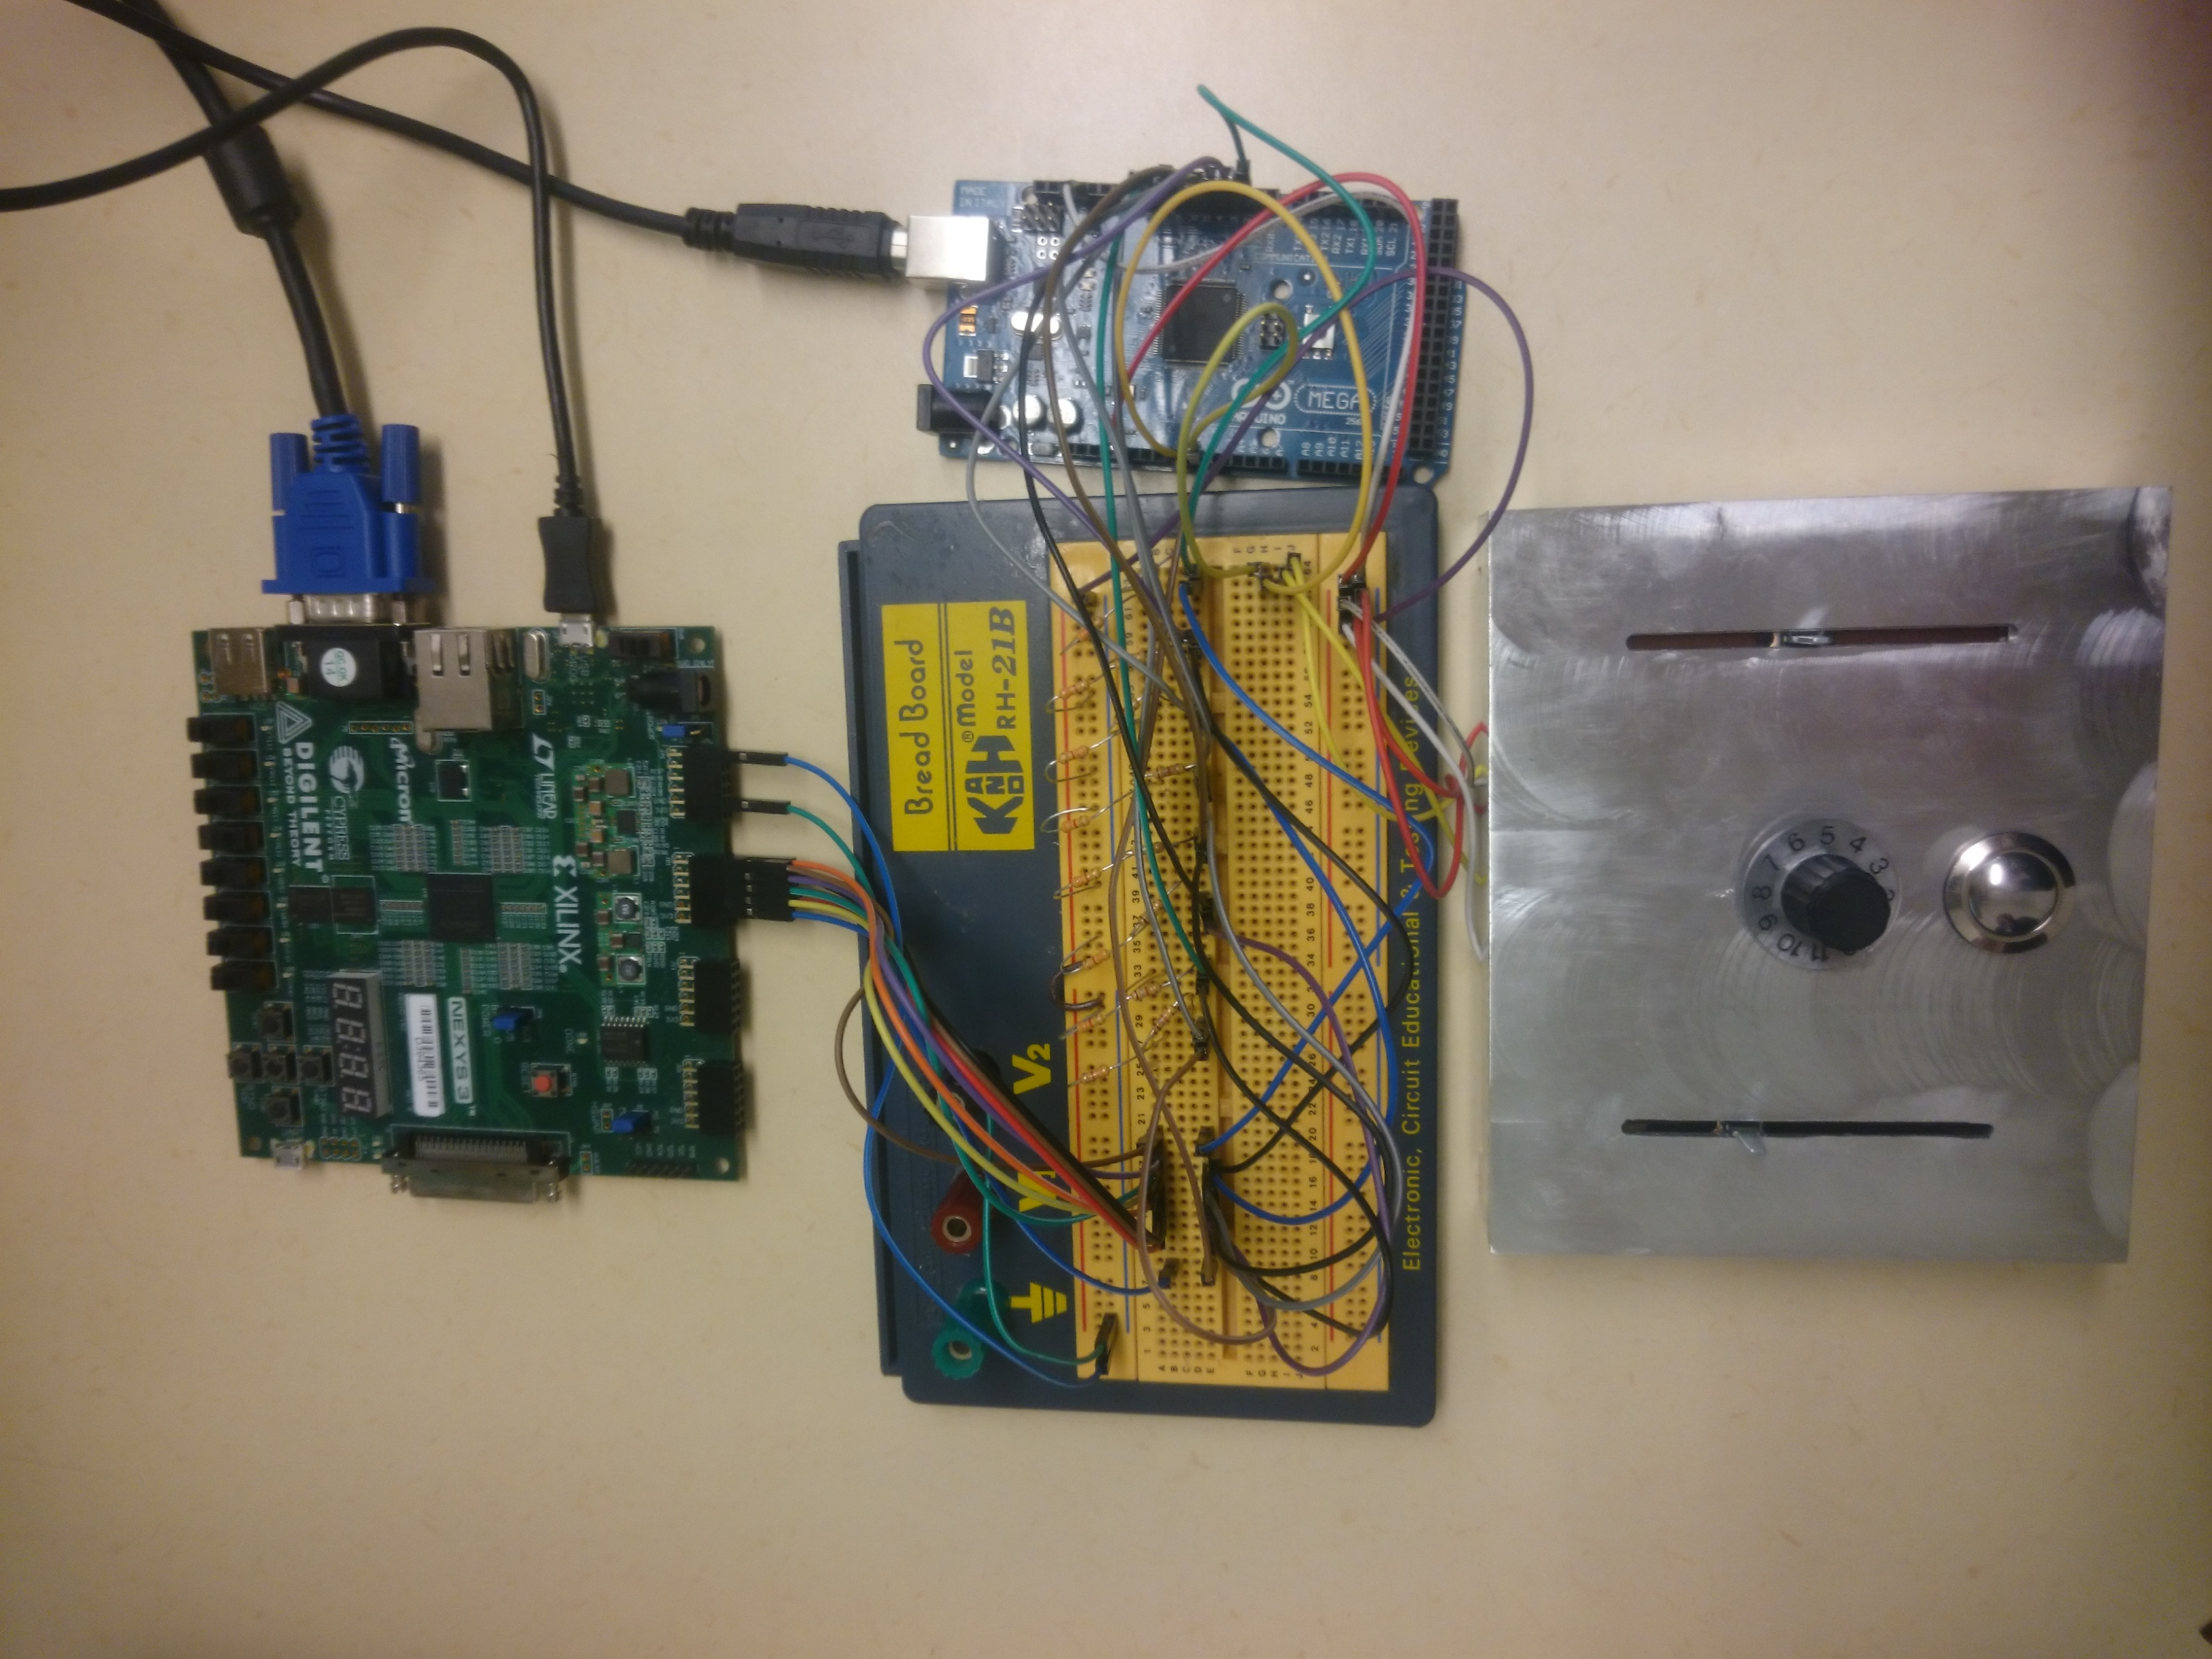
\includegraphics[scale=0.07]{../grafik/rapport-apparaten.JPG}
		\caption{Pong maskin}
		\label{fig:maskin}
	\end{figure}
\end{center}
\begin{center}
	\begin{figure}[H]
    	\centering
		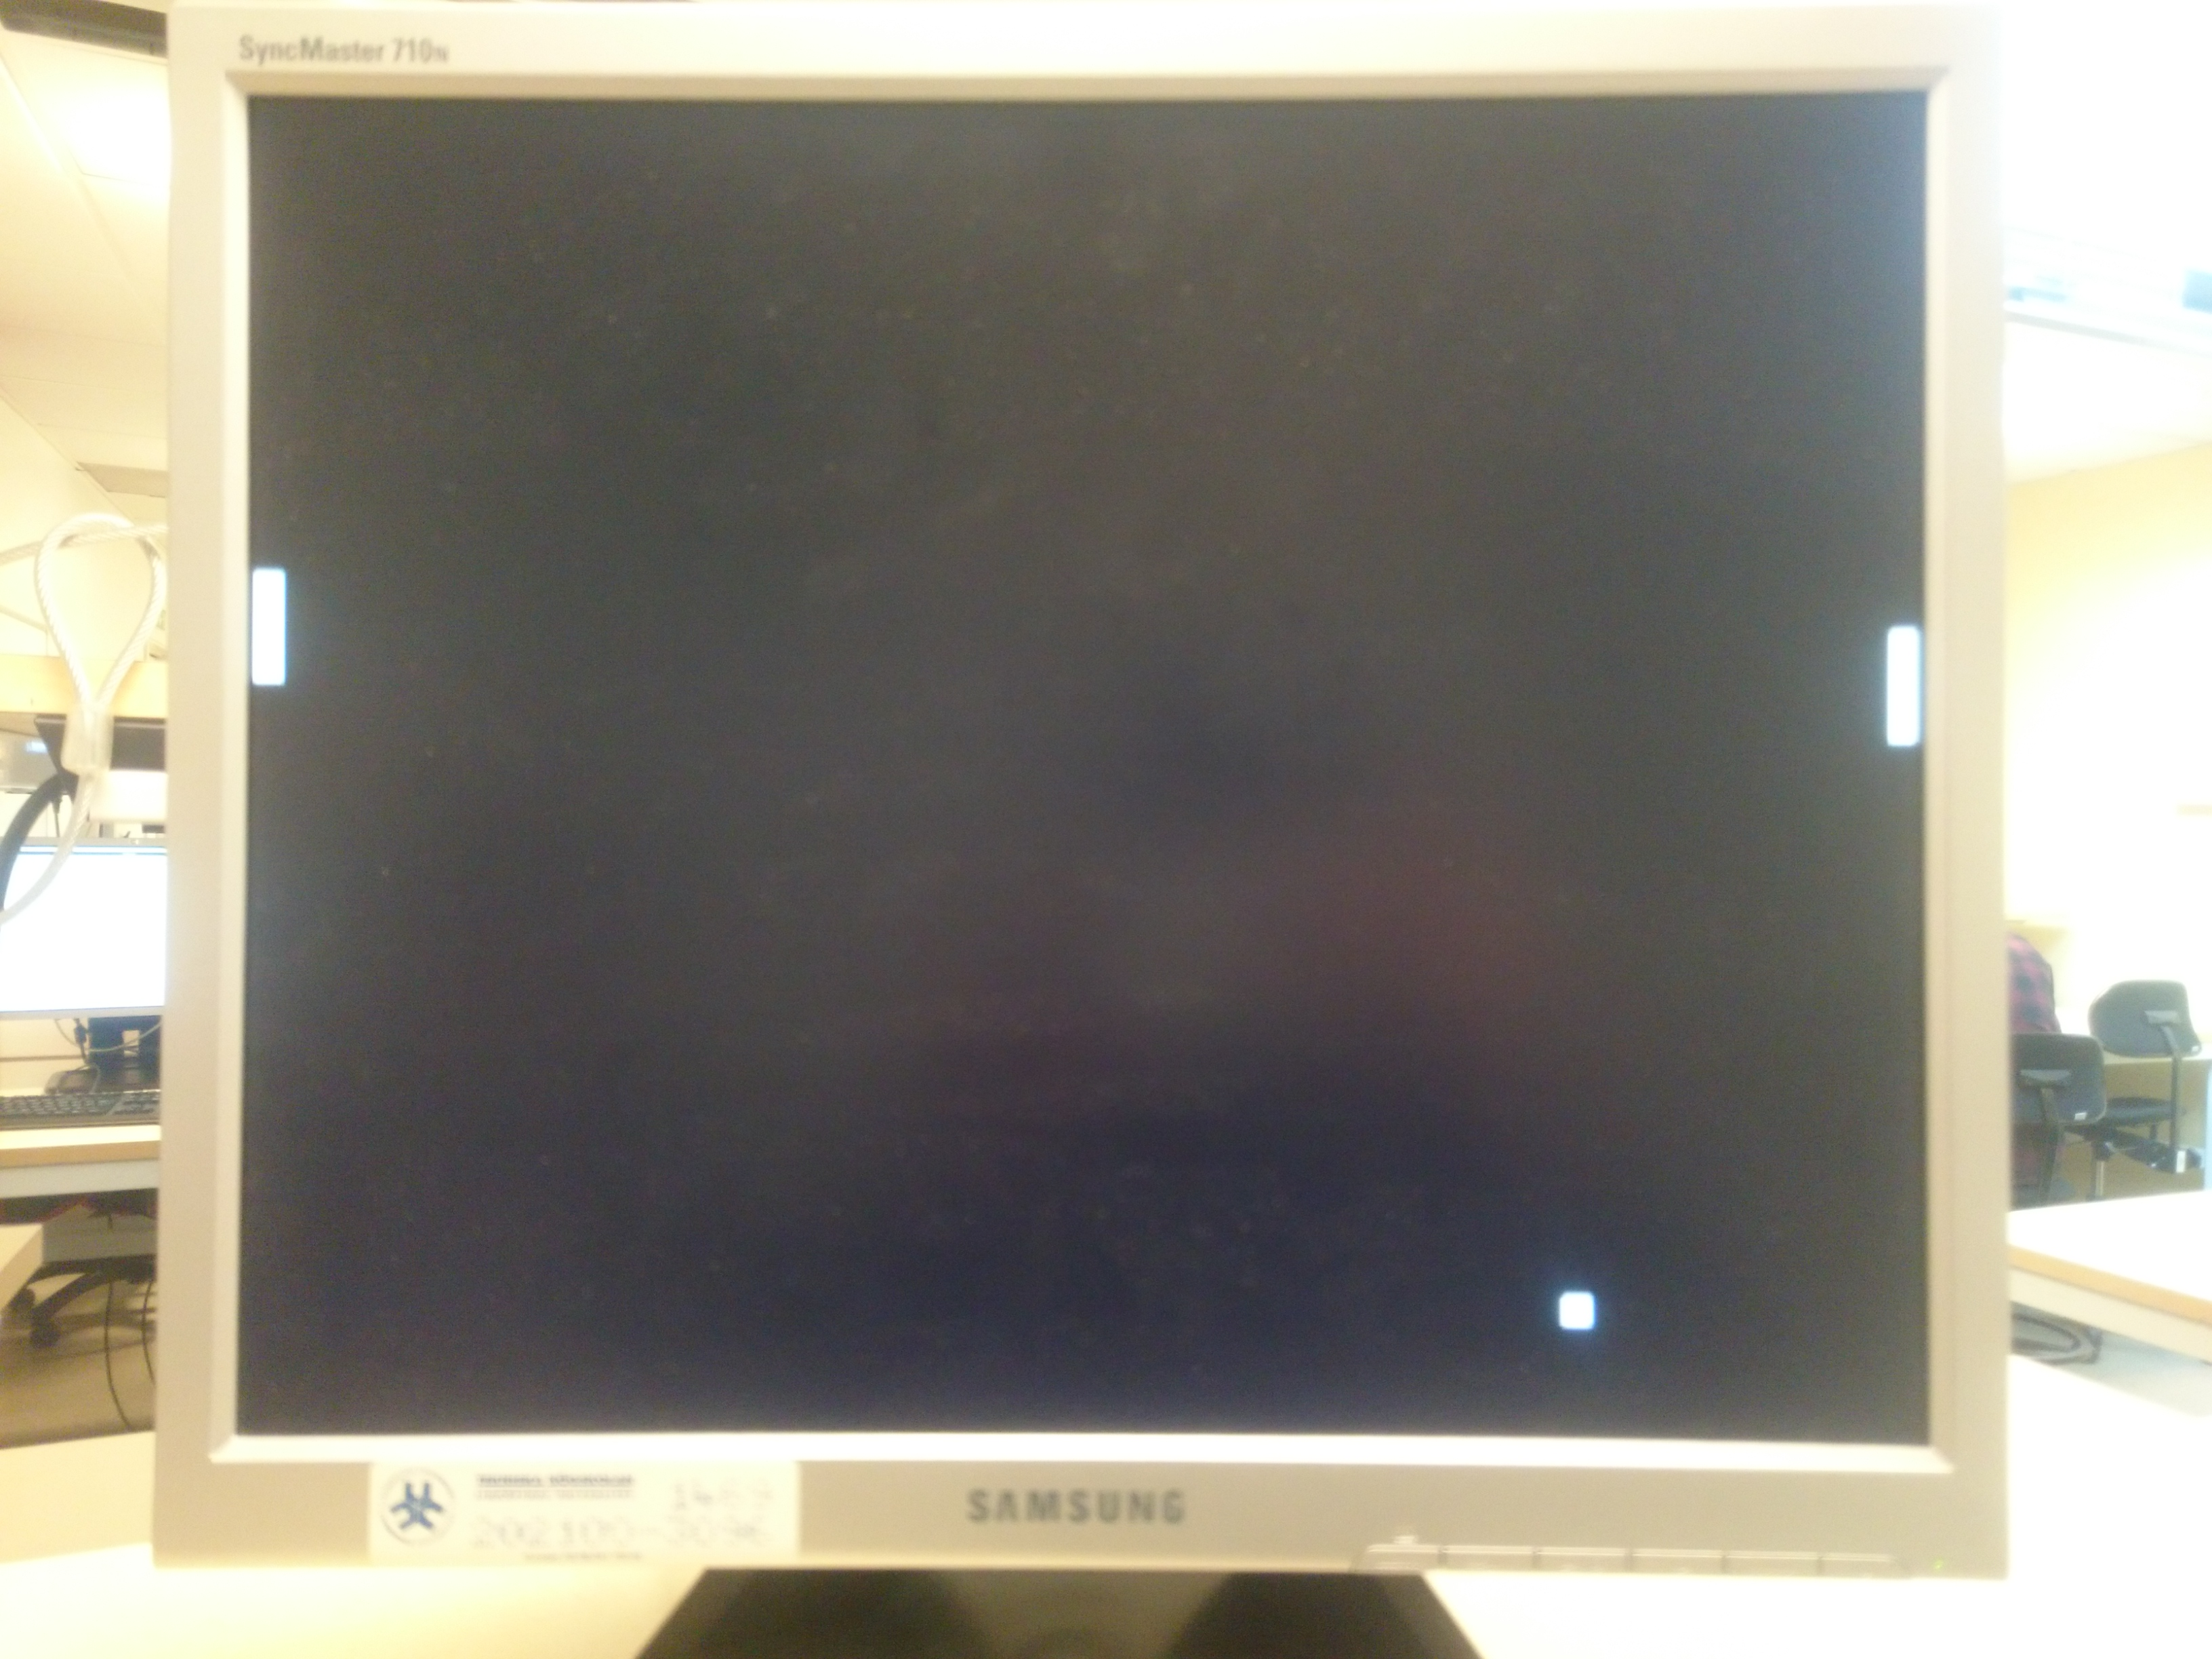
\includegraphics[scale=0.07]{../grafik/rapport-spel.JPG}
		\caption{VGA-Skärm}
		\label{fig:gui}
	\end{figure}
\end{center}

Två spelare använder varsin joystick som i sin tur styr spelarens stapel i spelet. Om någon av spelarna lyckas få bollen att passera motståndarens stapel får denna spelaren ett poäng som visas på toppen av skärmen. När en spelare fått tre poäng, vinner denna spelare och spelet startas om. Om man av någon anledning skulle vilja starta om innan en spelare fått tre poäng kan man använda en resetknapp, den svarta B8 knappen på Nexys-kortet.

